%%%%%%%%%%%%%%%%%%%%%%%%%%%%%%%%%%%%%%%%%%%%%%%
%%%This is a science homework template. Modify the preamble to suit your needs. 
%The junk text is   there for you to immediately see how the headers/footers look at first 
%typesetting.


\documentclass[12pt]{article}
\newcommand\independent{\protect\mathpalette{\protect\independenT}{\perp}}
\def\independenT#1#2{\mathrel{\rlap{$#1#2$}\mkern2mu{#1#2}}}
%AMS-TeX packages
\usepackage{amssymb,amsmath,amsthm} 
%geometry (sets margin) and other useful packages
\usepackage[margin=1.25in]{geometry}
\usepackage{graphicx,placeins}
\usepackage{float}

%
%Redefining sections as problems
%
\makeatletter
\newenvironment{problem}{\@startsection
       {section}
       {1}
       {-.2em}
       {-3.5ex plus -1ex minus -.2ex}
       {2.3ex plus .2ex}
       {\pagebreak[3]%forces pagebreak when space is small; use \eject for better results
       \large\bf\noindent{Problem }
       }
       }
       {%\vspace{1ex}\begin{center} \rule{0.3\linewidth}{.3pt}\end{center}}
       \begin{center}\large\bf \ldots\ldots\ldots\end{center}}
\makeatother


%
%Fancy-header package to modify header/page numbering 
%
\usepackage{fancyhdr}
\pagestyle{fancy}
%\addtolength{\headwidth}{\marginparsep} %these change header-rule width
%\addtolength{\headwidth}{\marginparwidth}
\lhead{Problem \thesection}
\chead{} 
\rhead{\thepage} 
\lfoot{\small\scshape Machine Learning in Complex Domains} 
\cfoot{} 
\rfoot{\footnotesize PS \#3} 
\renewcommand{\headrulewidth}{.3pt} 
\renewcommand{\footrulewidth}{.3pt}
\setlength\voffset{-0.25in}
\setlength\textheight{648pt}

%%%%%%%%%%%%%%%%%%%%%%%%%%%%%%%%%%%%%%%%%%%%%%%

%
%Contents of problem set
%    
\begin{document}

\title{MLCD 3: Posterior Inference}
\author{Mike Smith and Elan Hourticolon-Retzler}

\maketitle

\thispagestyle{empty}

%%%%%%%%%%%%%%%%%%%%%%%%%%%%%%%%%%%%%%%%%%%%%%%%%
\section*{2 Variational Inference - Mean-Field and Structured Mean-Field}
\noindent {\bf(2.1.a) Derivation of mean field given our network...}\\
For mean field, we are assuming an approximate distribution $Q = \prod_i Q(x_i)$, that is a product of marginals, to approximate our actual distribution $P$.  We also assume that $\forall i, \sum\limits_{x_i} Q(x_i) = 1$, that each marginal $Q(x_i)$ is a valid distribution in itself.\\
We want to optimize the energy functional, or minimize $\mathrm{KL}(q\|p)$.  The energy functional is as follows:
\begin{align*}
F &= \mathrm{E}_Q \ln P + \mathrm{H}_Q(X) \\
&= \mathrm{E}_Q \ln P + \mathrm{E}_Q \ln Q \\
&= \sum_{\phi \in \Phi} \mathrm{E}_Q [\ln \phi] + \mathrm{E}_Q \ln Q
\end{align*}
The first term is equal to the following, since $Q$ is a product of marginals:
\begin{equation*}
\mathrm{E}_Q \ln P = \mathrm{E}_{U_\phi \sim Q} [\ln \phi] = \sum_{u_\phi} Q(u_\phi) \ln \phi(u_\phi) = \sum_{u_\phi} \left( \prod_{X_i \in U_\phi } Q(x_i) \right) \ln \phi(u_\phi)
\end{equation*}
The second term, the entropy term, is equal to:
\begin{equation*}
\mathrm{H}_Q(X) = \mathrm{E}_Q \ln Q = \sum_i \mathrm{H}_Q(X_i)
\end{equation*}
We want to optimize the energy functional, subject to our given constraints, so we write a Lagrangian objective as follows, for each variable $i$:
\begin{align*}
L_i &= \sum_{\phi \in \Phi} \mathrm{E}_{U_\phi \sim Q} [\ln \phi] + \mathrm{H}_Q(X_i) + \lambda_i (\sum_{x_i} Q(x_i) = 1) \\
&= \sum_{\phi \in \Phi} \sum_{u_\phi} Q(u_\phi) \ln \phi(u_\phi) + \mathrm{H}_Q(X_i) + \lambda_i (\sum_{x_i} Q(x_i) = 1)
\end{align*}
We take the derivative with respect to one variable $x_i$ now. (We need to do this for each variable in turn, and optimize with respect to each variable.)  Since
\begin{equation*}
\frac{\delta }{\delta Q(x_i)} \mathrm{E}_{U_\phi \sim Q} [\ln \phi] = \mathrm{E}_{U_\phi \sim Q} [\ln \phi \mid x_i]
\end{equation*}
we have the derivative of the lagrangian as
\begin{equation*}
\frac{\delta L_i }{\delta Q(x_i)} = \sum_{\phi \in \Phi} \mathrm{E}_{U_\phi \sim Q} [\ln \phi \mid x_i] - \ln Q(x_i) - 1 + \lambda_i
\end{equation*}
Setting this derivative equal to 0 and rearranging terms we get:
\begin{equation*}
\ln Q(x_i) = \lambda - 1 + \sum_{\phi \in \Phi} \mathrm{E}_{U_\phi \sim Q} [\ln \phi \mid x_i]
\end{equation*}
Continuing to follow Koller p.450-452, we exponentiate both sides and renormalize; because $\lambda_i$ is a constant relative to $x_i$, it drops out when we renormalize, so we get:
\begin{equation*}
Q(x_i) = \frac{1}{Z_i} \mathrm{exp} \left\lbrace \sum_{\phi \in \Phi} \mathrm{E}_{U_\phi \sim Q} [\ln \phi \mid x_i] \right\rbrace
\end{equation*}
which is the equation that must hold if and only if $Q(X_i)$ is a local maximum of the mean field given $\lbrace Q(X_j) \rbrace_{j \not = i}$.  We note that if $X_i \not \in Scope(\phi)$ then $\mathrm{E}_{U_\phi \sim Q} [\ln \phi \mid x_i] = \mathrm{E}_{U_\phi \sim Q} [\ln \phi]$.  Put another way, expectations on such factors do not depend on $x_i$, and may therefore be lumped into the normalization constant $Z_i$.  We can therefore simplify and get:
\begin{equation*}
Q(x_i) = \frac{1}{Z_i} \mathrm{exp} \left\lbrace \sum_{\phi : X_i \in Scope(\phi)} \mathrm{E}_{(U_\phi - \lbrace X_i \rbrace) \sim Q} [\ln \phi(U_\phi , x_i)] \right\rbrace
\end{equation*}
Given our network for $P$, we see that we have factors over $(A)$, $(BA)$, $(CAB)$, $(DB)$, $(ECD)$, and $(FD)$.  We see from our previous simplification that the update equation for $Q(x_i)$ only sums over each factor $\phi$ such that $X_i$ is in $\phi$'s scope, lumping everything else into the normalization constant.  If we define $f(\phi, x_i) = \mathrm{E}_{(U_\phi - \lbrace X_i \rbrace) \sim Q} [\ln \phi(U_\phi , x_i)]$, we get the following update equations:
\begin{align*}
Q(a) &= \frac{1}{Z_a} \mathrm{exp} \left\lbrace f(A,a) + f(BA,a) + f(CAB,a) \right\rbrace \\
Q(b) &= \frac{1}{Z_b} \mathrm{exp} \left\lbrace f(DB,b) + f(BA,b) + f(CAB,b) \right\rbrace \\
Q(c) &= \frac{1}{Z_c} \mathrm{exp} \left\lbrace f(CAB,c) + f(ECD,c) \right\rbrace \\
Q(d) &= \frac{1}{Z_d} \mathrm{exp} \left\lbrace f(ECD,d) + f(DB,d) + f(FD,d) \right\rbrace \\
Q(e) &= \frac{1}{Z_e} \mathrm{exp} \left\lbrace f(ECD,e) \right\rbrace \\
Q(f) &= \frac{1}{Z_f} \mathrm{exp} \left\lbrace f(FD,f) \right\rbrace \\
\end{align*}
We now look at $f(\phi, x_i)$.
\[
f(\phi, x_i) = \mathrm{E}_{(U_\phi - \lbrace X_i \rbrace) \sim Q} [\ln \phi(U_\phi , x_i)] = \sum_{u_\phi \in (U_\phi - \lbrace X_i \rbrace)} Q(u_\phi) \ln \phi(u_\phi, x_i)
\]
We note that all variables are binary.  We can also see that in $\phi(u_\phi, x_i)$ we are considering only the sub-factor that has $X_i = x_i$, and we are summing over all other values $u_\phi$ of the other variables $(U_\phi - \lbrace X_i \rbrace)$, and multiplying by $Q(u_\phi)$, which is a product of marginals.  As a result, we arrived at the update equations in our 'inference.R' file.

\noindent \textbf{b - Implement and test mean field}\\
This does not look like a reasonable approximation, because we are losing many of the dependencies of the distribution.  The KL divergence is extremely high, signifying that Q is not a very close approximation for P.  Though we have optimized Q given this family of distributions, we should have chosen a different family.\\

\noindent \textbf{c - Derive structured mean field}\\
For structured mean field in our simple distribution, we are assuming the following about our family of Q's.
\[
Q(X_i) = Q(A,B,C,D,E,F) = \frac{1}{Z_Q} \Psi_1 (A,B,C) \Psi_2 (D,E,F)
\]
For reference, our set of factors for $P$ remains $\Phi = \lbrace A, BA, CAB, ECD, DB, FD\rbrace$.  From p458 of Koller, we have the energy functional:
\[
F\left[P_\Phi, Q\right] = \sum\limits_{k = 1}^{K} \mathrm{E}_Q (\ln \phi_k) - \sum\limits_{j = 1}^{J} \mathrm{E}_Q ( \ln \psi_j ) + \ln Z_Q
\]
We take the derivative, set equal to 0, and we obtain the update equation on p458, that $\psi_j$ is a stationary point if and only if the following holds:
\[
\psi_j(c_j) \propto \mathrm{exp} \left\lbrace \mathrm{E}_Q \lbrace \ln P_\Psi \mid c_j \rbrace - \sum_{k \not = j} \mathrm{E}_Q \lbrace \ln \psi_k \mid c_j \rbrace - F\left[P_\Phi, Q\right] \right\rbrace
\]
We note that the energy functional is independent of the current assignment $c_j$ so we can absorb it into the normalization constant, and we have:
\[
\psi_j(c_j) \propto \mathrm{exp} \left\lbrace \mathrm{E}_Q \lbrace \ln P_\Psi \mid c_j \rbrace - \sum_{k \not = j} \mathrm{E}_Q \lbrace \ln \psi_k \mid c_j \rbrace \right\rbrace
\]
As per p461 of Koller, we can simplify this further because of the marginal independencies in Q.  Expectations with respect to variables that aren't in the scope of $C_j$ add a constant amount to all expectations, so can be absorbed into the normalization constant.  We get, therefore:
\begin{multline*}
\psi_j(c_j) \propto \mathrm{exp} \left\lbrace \sum_{\phi \in A_j} \mathrm{E}_{X \sim Q} \left[ \ln \phi \mid c_j \right] - \sum_{\psi_k \in B_j} \mathrm{E}_{X \sim Q} \lbrace \ln \psi_k \mid c_j \rbrace \right\rbrace \\
A_j = \lbrace \phi \in \Phi : Q \not \models (U_\phi \independent C_j)\rbrace \\ 
B_j = \lbrace \psi \in \Psi : Q \not \models (C_k \independent C_j)\rbrace - \lbrace
 C_j \rbrace \\
\end{multline*}
We note that in our simple example, the set $B_j$ is empty for both structures ABC, DEF.  We see that $A_j$ is the set of all factors such that Q does not say they are independent from the variables in $\psi_j$.  Let $ g(\phi, c_j) = \sum_{u_\phi} Q(u_\phi \mid c_j) \ln \phi(u_\phi)$.  We note that the terms $Q(u_\phi \mid c_j)$ may equal marginal probabilities, marginalizing out all variables in the sepset $u_\phi - c_j$.  We get as update equations, therefore:
\begin{align*}
\psi_{ABC}(c_{abc}) &= \mathrm{exp} \lbrace g(A, abc) + g(BA, abc) + g(ABC,abc) + g(ECD, abc) + g(DB,abc) \rbrace \\ 
\psi_{DEF}(c_{def}) &= \mathrm{exp} \lbrace g(DB, def) + g(ECD, def) + g(FD,def) \rbrace \\ 
\end{align*}

\noindent \textbf{d - Implement and test structured mean field}\\
This does look like a better approximation than mean field.  It is encapsulating dependencies between A, B, and C, and between D, E, and F, as opposed to assuming they are all independent.  This more closely approximates our true distribution P.  The smaller KL divergence means it's closer to P.  Structured mean field performs better for this network because it's simple, and there are very clear dependencies.  We chose structures / clusters / groups of variables such that we capture some of these dependencies, and this of course will be better than simply assuming everything is indepdendent of everything else, as in mean field.  

%%%%%%%%%%%%%%%%%%%%%%%%%%%%%%%%%%%%%%%%%%%%%%%%%
\section*{3 Analyzing Multiple Text Corpora}
\noindent {\bf(a) Problem details...}\\

%%%%%%%%%%%%%%%%%%%%%%%%%%%%%%%%%%%%%%%%%%%%%%%%%
\section*{4 Collapsed Gibbs Sampler Implementation}
\noindent {\bf(a) See output files...}\\

%%%%%%%%%%%%%%%%%%%%%%%%%%%%%%%%%%%%%%%%%%%%%%%%%
\section*{5 Blocked Gibbs Sampler}
\noindent {\bf(5.1) Analysis Questions}\\
Given the full expanded form of the likelihood:\\
\begin{align}
P (z, x, c, w\mid \alpha, \beta, \lambda) &= P (w \mid z, x, c, \beta)P (z\mid \alpha)P(x\mid \lambda) \nonumber\\
&=\prod_{k}(\frac{\Gamma(\sum_{w} \beta)}{\Gamma(\sum_{w} n^{k}_{w}+\beta)} \prod_{w} \frac{\Gamma(n^{k}_{w}+\beta))}{\Gamma(\beta)} )\nonumber\\
&\times \prod_{c}\prod_{k}(\frac{\Gamma(\sum_{w} \beta)}{\Gamma(\sum_{w} n^{c,k}_{w}+\beta))} \prod_{w} \frac{\Gamma(n^{c,k}_{w}+\beta))}{\Gamma(\beta)} )\nonumber\\
&\times \prod_{d}(\frac{\Gamma(\sum_{k} \alpha)}{\Gamma(\sum_{k} n^{d}_{k}+\alpha)} \prod_{k} \frac{\Gamma(n^{d}_{k}+\alpha))}{\Gamma(\alpha)} ) \times \prod_{(d,i)} P(x_{d,i} \mid \lambda)\nonumber\\
\end{align}

\begin{align}
P (z_{d,i}, x_{d,i} \mid z-z_{d,i},x-x_{d,i},c,w;\alpha, \beta, \lambda) &= \frac{P (z, x, c, w\mid \alpha, \beta, \lambda)}{P (z-z_{d,i}, x-x_{d,i}, c, w\mid \alpha, \beta, \lambda)} \nonumber\\
\end{align}

\begin{align}
P &(z_{d,i}=k, x_{d,i} = 0 \mid z-z_{d,i},x-x_{d,i},c,w;\alpha, \beta, \lambda)  \nonumber\\
&=\frac{\frac{\Gamma(n^{k}_{w_{d,i}} +1+\beta)}{\Gamma(1+\sum_{w} n^{k}_{w}+\beta)}  \frac{\Gamma(n^{d}_{k} +1+\alpha)}{\Gamma(1+\sum_{k'} n^{k'}_{w}+\alpha)}}{\frac{\Gamma(n^{k}_{w_{d,i}} +\beta)}{\Gamma(\sum_{w} n^{k}_{w}+\beta)}  \frac{\Gamma(n^{d}_{k} +\alpha)}{\Gamma(\sum_{k'} n^{k'}_{w}+\alpha)}} P(x_{d,i} = 0 \mid \lambda)\nonumber\\
&= \frac{n^{k}_{w_{d,i}}+\beta}{n^{k}_{*}+V\beta}  \frac{n^{d}_{k} +\alpha}{n^{d}_{*} +K\alpha} (1-\lambda) 
\end{align}

\begin{align}
P &(z_{d,i}=k, x_{d,i} = 1 \mid z-z_{d,i},x-x_{d,i},c,w;\alpha, \beta, \lambda)  \nonumber\\
&=\frac{\frac{\Gamma(n^{c,k}_{w_{d,i}} +1+\beta)}{\Gamma(1+\sum_{w} n^{c,k}_{w}+\beta)}  \frac{\Gamma(n^{d}_{k} +1+\alpha)}{\Gamma(1+\sum_{k'} n^{k'}_{w}+\alpha)}}{\frac{\Gamma(n^{c,k}_{w_{d,i}} +\beta)}{\Gamma(\sum_{w} n^{c,k}_{w}+\beta)}  \frac{\Gamma(n^{d}_{k} +\alpha)}{\Gamma(\sum_{k'} n^{k'}_{w}+\alpha)}} P(x_{d,i} = 1 \mid \lambda)\nonumber\\
&= \frac{n^{c,k}_{w_{d,i}}+\beta}{n^{c,k}_{*}+V\beta}  \frac{n^{d}_{k} +\alpha}{n^{d}_{*} +K\alpha} (\lambda) 
\end{align}


%%%%%%%%%%%%%%%%%%%%%%%%%%%%%%%%%%%%%%%%%%%%%%%%%
\section*{6 Text Analysis with MCLDA}

\noindent{\bf Note:} Since our test data is much shorter than our training data it's likelihood is naturally much higher. A possibly more informative metric would have been log likelihood per word.\\
\\
\noindent {\bf(1)} For each chain the training likelihood increases (monotonically, save for minor fluctuations)  till it plateaus around 300 iterations. Similarly the likelihood for test data decreases till it plateaus however with much more variation. \\

\begin{figure}[H]
\centering
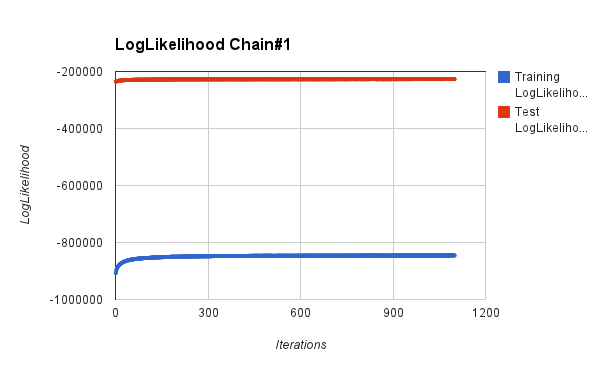
\includegraphics[keepaspectratio=true,scale=0.8]{charts/chain1}
\label{chain1}
\end{figure}

\begin{figure}[H]
\centering
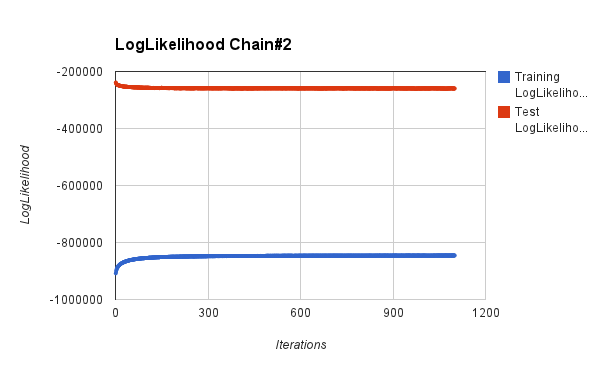
\includegraphics[keepaspectratio=true,scale=0.8]{charts/chain2}
\label{chain2}
\end{figure}

\begin{figure}[H]
\centering
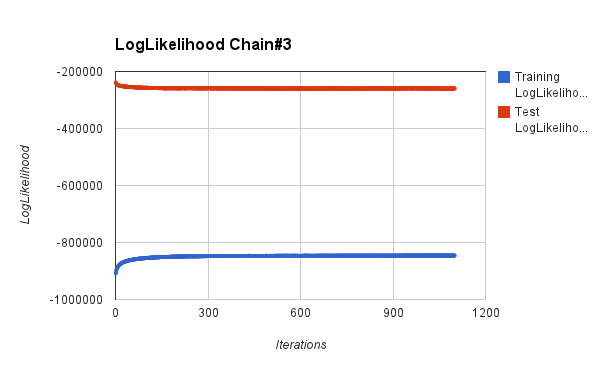
\includegraphics[keepaspectratio=true,scale=0.8]{charts/chain3}
\label{chain3}
\end{figure}

\begin{figure}[H]
\centering
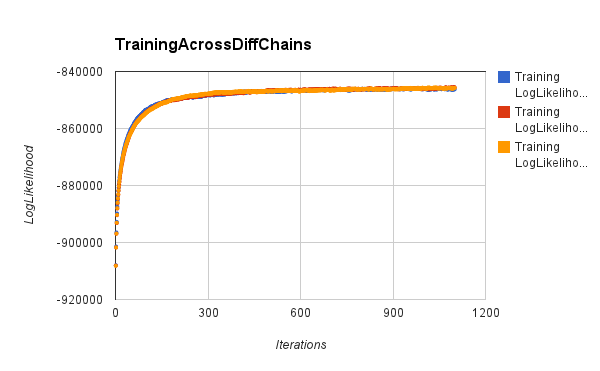
\includegraphics[keepaspectratio=true,scale=0.8]{charts/trainingLLOfChains}yo
\label{chainTraining}
\end{figure}

\begin{figure}[H]
\centering
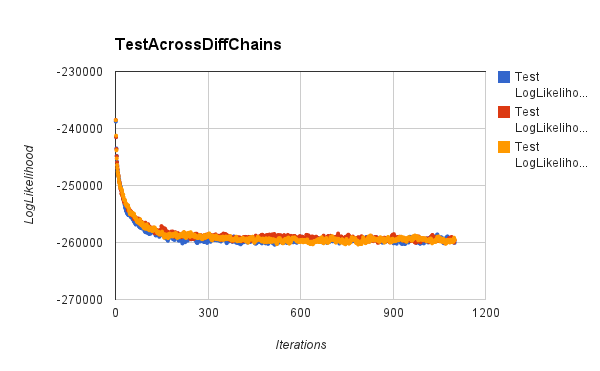
\includegraphics[keepaspectratio=true,scale=0.8]{charts/testLLOfChains}
\label{chainTest}
\end{figure}

\noindent {\bf(4)} \\
\begin{figure}[H]
\centering
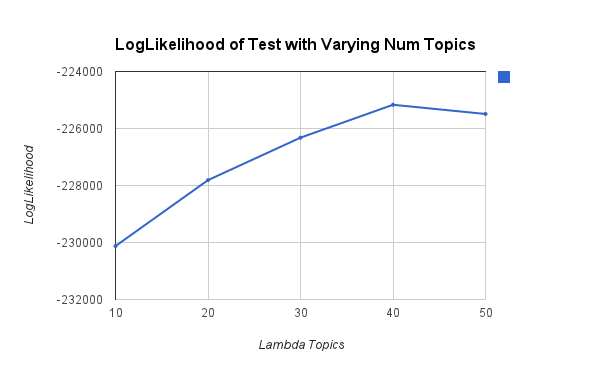
\includegraphics[keepaspectratio=true,scale=0.8]{charts/VaryingKonTest}
\label{kVariation}
\end{figure}

\noindent {\bf(5)}\\
\begin{figure}[H]
\centering
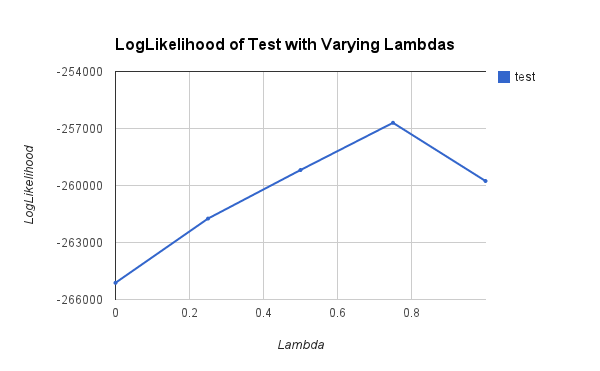
\includegraphics[keepaspectratio=true,scale=0.8]{charts/VaryingLambdaOnTest}
\label{lambdaVariation}
\end{figure}

\noindent {\bf(6)}  \\
\noindent {\bf(a)} As we increase K we allow topics to become more and more specific meaning that we can label individual documents with a much higher granularity increasing the log likelihood. This greatly increases our likelihood on test data to a point (around K=40) afterwards we start overfitting the training data and our rate begins to drop off again. \\
\\
\noindent {\bf(b)} Varying $\lambda$ controls the amount we sample from global vs corpus dependent distribution of topics. Test performance increases with $\lambda$ initially but then peaks around .75 before decreasing again. This implies that there is an optimal lambda that is between always sampling from the global and always sampling from collection dependent. This intuitively makes sense because with $\lambda = 0$ this would imply that there is no advantage of looking at collection specific topics. In the other extreme with $\lambda=1$ would imply that there was no benefit to generalizing and considering global topics. Everywhere in between implies that there are differences in which words each collection uses to describe a topic but there is still a benefit to considering the generalized corpus. Our data show that between these two scenarios we much heavily prefer using the collection dependent distributions.   \\
\\
\noindent {\bf(c)} $\alpha$ controls how much we smooth our topic distribution for each document, $\theta$. $\beta$ controls how much we smooth our topics for each word ($\phi$). When $\alpha$ is large this means that each document ends up contributing its bag of words more heavily to every topics smoothing the overall distributions. Similarly when $\beta$ is large the distributions are forced to be much more uniform.  In practice, this results in topics that are less discernible and less likely to represent a more specific topic as we understand the meaning of the word. \\

\begin{figure}[H]
\centering
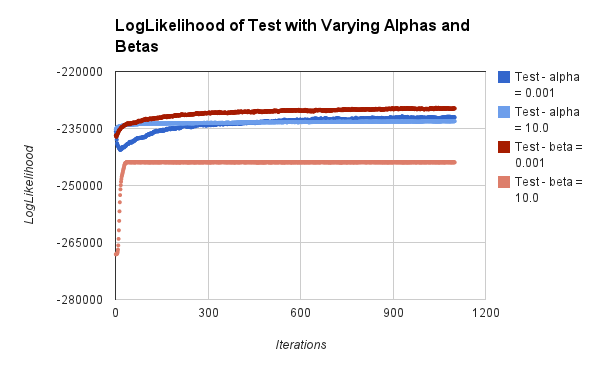
\includegraphics[keepaspectratio=true,scale=0.8]{charts/VaryingAlphasBetasOnTest}
\label{alphaBetaVariation}
\end{figure}

%%%%%%%%%%%%%%%%%%%%%%%%%%%%%%%%%%%%%%%%%%%%%%%%%
\section*{7 Variational Inference}
\noindent {\bf(7.1) Derivation}\\
We wish to derive the update equations for variational inference, as computing $p(\theta, c, \phi, z, x \mid w, \alpha, \beta, \lambda)$ for exact inference is intractable.  By definition of a conditional probability we have:
\begin{equation*}
\frac{p(\theta, c, \phi, z, x, w, \mid \alpha, \beta, \lambda)}{p(w \mid \alpha, \beta, \lambda)}
\end{equation*}
From the graphical model of our distribution at the top of page 6 of the homework PDF, it is easy to mutilate the graph of P to arrive at a more tractable family of approximate Q distributions.  We omit the $w$ node, and omit the edges between $\theta$, $z$, $\phi$, and $x$.  We also introduce free variational parameters $\gamma$, $\delta$, $\zeta$, and $\eta$ respectively on our factors of Q, themselves distributions.  $q(\theta \mid \gamma) \sim \mathrm{Dirichlet}(\gamma)$, $q(z \mid \delta) \sim \mathrm{Multinomial}(\delta)$, $q(\phi \mid \zeta) \sim \mathrm{Dirichlet}(\zeta)$, and $q(x \mid \eta) \sim \mathrm{Bernoulli}(\eta)$.\\
We note that we want to minimize the KL Divergence from $q$ to $p$, which is
\begin{equation*}
\mathrm{KL}(q\|p) = \ln(Z) - \mathrm{E}_q (\log \widetilde{p}) - \mathrm{E}_q (\log q) 
\end{equation*}
and this is equivalent to maximizing the energy functional:
\begin{equation*}
F = \mathrm{E}_q (\log \widetilde{p}) + \mathrm{E}_q (\log q)
\end{equation*}
We know that our joint of $\widetilde{p}$ factorizes as the following:
\begin{equation*}
\widetilde{p}(\theta, c, \phi, z, x, w, \mid \alpha, \beta, \lambda) = p(z \mid \theta) p(\theta \mid \alpha) p(x \mid \lambda) p(\phi \mid \beta) p(w \mid z, x, c, \phi)
\end{equation*}
and that $p(w \mid z, x, c, \phi)$ factorizes as the following:
\begin{equation*}
p(w \mid z, x, c, \phi) = \prod_{(d,i)} ( p(w_{d,i} \mid \phi_k)^{I(x_{d,i} = 0)} p(w_{d,i} \mid \phi_{k}^{c_0})^{I(x_{d,i} = 1, c= 0)} p(w_{d,i} \mid \phi_{k}^{c_1})^{I(x_{d,i} = 1, c= 1)})
\end{equation*}
and that $q$ factorizes\ as the following:
\begin{equation*}
q(\theta, z, \phi, x \mid \gamma, \delta, \zeta, \eta) = q(\theta \mid \gamma) \prod_d q(z \mid \delta) q(\phi \mid \zeta) q(x \mid \eta)
\end{equation*}
so we can plug these into our definition of the energy functional.
\begin{align*}
F &= \mathrm{E}_q \{\log p(z \mid \theta) + \log p(\theta \mid \alpha) + \log p(x \mid \lambda) + \log p(\phi \mid \beta) \\
&+ \log p(w \mid z, x, c, \phi) \\
&+ \mathrm{E}_q \{ \log q(\theta \mid \gamma) + \sum_d \left( \log q(z \mid \delta) + \log q(\phi \mid \zeta) + \log q(x \mid \eta) \right) \} 
\end{align*}
Now, we can calculate the individual terms by taking the logarithm of each, also moving the expectation to each term, as the expectation of a sum is the sum of expectations.  We note that $q(\theta \mid \gamma) \sim \mathrm{Dirichlet}(\gamma)$, $q(z \mid \delta) \sim \mathrm{Multinomial}(\delta)$, $q(\phi \mid \zeta) \sim \mathrm{Dirichlet}(\zeta)$, $q(x \mid \eta) \sim \mathrm{Bernoulli}(\eta)$, and we consider only the update equations given a specific document, as the source did.\\
\noindent \textit{Note that some of these equations were taken from\\ http://machinelearning.wustl.edu/mlpapers/paper\_files/BleiNJ03.pdf \\ We cite their derivations.}
\begin{align*}
\mathrm{E}_q \log p(z \mid \theta) &= \sum\limits_{i=1}^{N_d} \sum\limits_{k=1}^K \delta_{i,k}(\Psi(\gamma_k) - \Psi(\sum_{j=1}^k \gamma_j) ) \\
\mathrm{E}_q\log p(\theta \mid \alpha) &= \log \Gamma (K \alpha) - \sum\limits_{k=1}^K \log \Gamma(\alpha) + \sum\limits_{k=1}^K (\alpha - 1)(\Psi(\gamma_k) - \Psi(\sum_{j=1}^K \gamma_j) )\\
\mathrm{E}_q\log p(x \mid \lambda) &= I(x=0) Q(x=0|\eta) \log \lambda + I(x=1) Q(x=1|\eta) \log (1-\lambda) \\
\mathrm{E}_q\log p(\phi \mid \beta) &= I(x=0)(\log \Gamma (K \beta) - \sum\limits_{k=1}^V \log \Gamma(\beta) + \sum\limits_{k=1}^V (\beta - 1)(\Psi(\zeta_k) - \Psi(\sum_{j=1}^V \zeta_j) ))\\
&+ I(x=1,c=0)(\log \Gamma (K \beta) - \sum\limits_{k=1}^V \log \Gamma(\beta) + \sum\limits_{k=1}^V (\beta - 1)(\Psi(\zeta_k) - \Psi(\sum_{j=1}^V \zeta_j) ))\\
&+ I(x=1,c=1)(\log \Gamma (K \beta) - \sum\limits_{k=1}^V \log \Gamma(\beta) + \sum\limits_{k=1}^V (\beta - 1)(\Psi(\zeta_k) - \Psi(\sum_{j=1}^V \zeta_j) ))\\
\mathrm{E}_q\log p(w \mid z, x, c, \phi) &= \sum_{d,i} \lbrace q(w_{d,i} \mid \phi_k)^{I(x_{d,i} = 0)} q(w_{d,i} \mid \phi_{k}^{c_0})^{I(x_{d,i} = 1, c= 0)} q(w_{d,i} \mid \phi_{k}^{c_1})^{I(x_{d,i} = 1, c= 1)} \\ 
& \times [ I(x_{d,i} = 0) (\log p(w_{d,i} \mid \phi_z)) + I(x_{d,i} = 1, c= 0) (\log p(w_{d,i} \mid \phi_{z}^{c_0}) \\
& + I(x_{d,i} = 1, c= 1) (\log p(w_{d,i} \mid \phi_{z}^{c_1})) ] \rbrace \\
\mathrm{E}_q\log q(\theta \mid \gamma) &= \log \Gamma (\sum\limits_{k=1}^K \gamma_k) - \sum\limits_{k=1}^K \log \Gamma(\gamma_k) + \sum\limits_{k=1}^K (\gamma_k - 1)(\Psi(\gamma_k) - \Psi(\sum_{j=1}^K \gamma_j) )\\
\mathrm{E}_q\log q(z \mid \delta) &= \sum\limits_{i=1}^{N_d} \sum\limits_{k=1}^K \delta_{i,k} \log \delta_{i,k} \\
\mathrm{E}_q\log q(\phi \mid \zeta) &= I(x=0)(\log \Gamma (K \zeta) - \sum\limits_{k=1}^V \log \Gamma(\zeta) + \sum\limits_{k=1}^V (\zeta - 1)(\Psi(\zeta_k) - \Psi(\sum_{j=1}^V \zeta_j) ))\\
&+ I(x=1,c=0)(\log \Gamma (K \zeta) - \sum\limits_{k=1}^V \log \Gamma(\zeta) + \sum\limits_{k=1}^V (\zeta - 1)(\Psi(\zeta_k) - \Psi(\sum_{j=1}^V \zeta_j) ))\\
&+ I(x=1,c=1)(\log \Gamma (K \zeta) - \sum\limits_{k=1}^V \log \Gamma(\zeta) + \sum\limits_{k=1}^V (\zeta - 1)(\Psi(\zeta_k) - \Psi(\sum_{j=1}^V \zeta_j) ))\\
\mathrm{E}_q\log q(x \mid \eta) &= I(x=0) Q(x=0|\eta) \log \eta + I(x=1) Q(x=1|\eta) \log (1-\eta) \\
\end{align*}
We now need to define four update equations for $Q$, one each for $\gamma_{d,k}$, $\delta_{d,i}$, $\zeta_{k,w}$, and $\eta_{d,i}$.  For each variable, we form the Langrangian by collecting terms involving that variable and adding the constraints of that variable.  We'll take the derivative with respect to variable $i$ and set that to zero, rearrange, and exponentiate.
\begin{align*}
L_{\gamma_{k}} &= \delta_{i,k}(\Psi(\gamma_k) - \Psi(\sum_{j=1}^k \gamma_j) ) + (\alpha - 1)(\Psi(\gamma_k) - \Psi(\sum_{j=1}^k \gamma_j) ) \\ 
&+ \log \Gamma (\sum\limits_{k=1}^K \gamma_k) - \sum\limits_{k=1}^K \log \Gamma(\gamma_k) + \sum\limits_{k=1}^K (\gamma_k - 1)(\Psi(\gamma_k) - \Psi(\sum_{j=1}^K \gamma_j) ) \\ 
L_{\delta_{i,k}} &= \delta_{i,k}(\Psi(\gamma_k) - \Psi(\sum_{j=1}^k \gamma_j) ) + \delta_{i,k} \log \delta_{i,k} \\
L_{\zeta_{k,w}} &= asdf \\
L_{\eta_{i}} &= I(x=0) Q(x=0|\eta) \log \lambda + I(x=1) Q(x=1|\eta) \log (1-\lambda) \\
&+ I(x=0) Q(x=0|\eta) \log \eta + I(x=1) Q(x=1|\eta) \log (1-\eta)
\end{align*}
Therefore, the update equations are the following:
\begin{align*}
\mathrm{Update}_{Q_\gamma} &= asdf \\ 
\mathrm{Update}_{Q_\delta} &= asdf \\
\mathrm{Update}_{Q_\zeta} &= asdf \\
\mathrm{Update}_{Q_\eta} &= asdf 
\end{align*}


%%%%%%%%%%%%%%%%%%%%%%%%%%%%%%%%%%%%%%%%%%%%%%%%%

%%%%%%%%%%%%%%%%%%%%%%%%%%%%%%%%%%%%%%%%%%%%%%%%%
\end{document}
